\documentclass[12pt]{article}
\usepackage{amssymb,amsmath,setspace,graphicx,url,hyperref}
\hypersetup{hidelinks}
\usepackage[labelfont=bf]{caption}
\usepackage[left=.9in,right=.9in,top=1in,bottom=0.75in]{geometry}
\setstretch{1.5}
%% Auto-generated by A2-reduced-form.do — do not edit by hand
\newcommand{\eventStudyCoef}{0.056}
\newcommand{\eventStudyBaseRate}{0.194}
\newcommand{\eventStudyBaseRateCond}{1.061}
\newcommand{\eventStudyPctReduction}{29}
\newcommand{\eventStudyPctReductionCond}{5}

%% Auto-generated by O2-structural-summary.do — do not edit by hand
\newcommand{\reallocationMeanMyopic}{39.6}
\newcommand{\healthFXMeanMyopic}{0.5}
\newcommand{\nHRRsMyopic}{280}
\newcommand{\nAlphaZeroMyopic}{51}
\newcommand{\alphaDistRatioMyopic}{2.9}
\newcommand{\nHRRsEtaFiveMyopic}{281}
\newcommand{\reallocationMeanFullFamMyopic}{40.0}
\newcommand{\healthFXMeanFullFamMyopic}{0.4}
\newcommand{\partialFXNonzeroMyopic}{3.4}
\newcommand{\partialFXAllMyopic}{2.5}
\newcommand{\reallocationMeanFWD}{32.1}
\newcommand{\healthFXMeanFWD}{0.4}
\newcommand{\nHRRsFWD}{277}
\newcommand{\nAlphaZeroFWD}{46}
\newcommand{\alphaDistRatioFWD}{3.8}
\newcommand{\nHRRsEtaFiveFWD}{279}
\newcommand{\reallocationMeanFullFamFWD}{35.0}
\newcommand{\healthFXMeanFullFamFWD}{0.4}
\newcommand{\partialFXNonzeroFWD}{3.0}
\newcommand{\partialFXAllFWD}{2.0}

%% Auto-generated by A2b-rereferral.do
\newcommand{\rereferEvents}{1190521}
\newcommand{\rereferFailures}{112871}
\newcommand{\rereferBase}{0.160}
\newcommand{\rereferFX}{-0.0110}
\newcommand{\rereferSE}{0.0011}
\newcommand{\rereferPct}{-6.8}
\newcommand{\rereferFXpcp}{-0.0106}
\newcommand{\rereferSEpcp}{0.0011}
\newcommand{\rereferFXhistzero}{-0.0126}
\newcommand{\rereferSEhistzero}{0.0013}
\newcommand{\rereferBasehistzero}{0.059}
\newcommand{\rereferPcthistzero}{-21.2}
\newcommand{\rereferFXhistone}{-0.0100}
\newcommand{\rereferSEhistone}{0.0018}
\newcommand{\rereferBasehistone}{0.131}
\newcommand{\rereferPcthistone}{-7.6}
\newcommand{\rereferFXhisttwo}{-0.0093}
\newcommand{\rereferSEhisttwo}{0.0026}
\newcommand{\rereferBasehisttwo}{0.281}
\newcommand{\rereferPcthisttwo}{-3.3}
\newcommand{\shareThreeBase}{0.154}
\newcommand{\shareThreeFX}{-0.0083}
\newcommand{\shareThreeSE}{0.0007}
\newcommand{\rereferESPost}{-0.0063}
\newcommand{\rereferESPostSE}{0.0011}
\newcommand{\rereferESPre}{-0.0022}
\newcommand{\rereferESPreSE}{0.0011}
\newcommand{\rereferESFirst}{-0.0108}
\newcommand{\rereferESFirstSE}{0.0014}
\newcommand{\rereferESBase}{0.151}
\newcommand{\rereferESPosthistzero}{-0.0083}
\newcommand{\rereferESPostSEhistzero}{0.0006}
\newcommand{\rereferESPosthistone}{-0.0147}
\newcommand{\rereferESPostSEhistone}{0.0019}
\newcommand{\rereferESPosthisttwo}{-0.0039}
\newcommand{\rereferESPostSEhisttwo}{0.0026}

% From Rereferral_Checks_1_1_0.csv (check "sutva"); A2b does not yet write these as macros.
\newcommand{\rereferESEventsSutva}{279,867}
\newcommand{\rereferESFailuresSutva}{17,562}
\newcommand{\rereferESFirstSutva}{-0.0146}
\newcommand{\rereferESFirstSESutva}{0.0050}

% Replacement for Section 2 of learning-draft.tex (failure-versus-success re-referral design).
% To swap in: add %% Auto-generated by A2b-rereferral.do
\newcommand{\rereferEvents}{1190521}
\newcommand{\rereferFailures}{112871}
\newcommand{\rereferBase}{0.160}
\newcommand{\rereferFX}{-0.0110}
\newcommand{\rereferSE}{0.0011}
\newcommand{\rereferPct}{-6.8}
\newcommand{\rereferFXpcp}{-0.0106}
\newcommand{\rereferSEpcp}{0.0011}
\newcommand{\rereferFXhistzero}{-0.0126}
\newcommand{\rereferSEhistzero}{0.0013}
\newcommand{\rereferBasehistzero}{0.059}
\newcommand{\rereferPcthistzero}{-21.2}
\newcommand{\rereferFXhistone}{-0.0100}
\newcommand{\rereferSEhistone}{0.0018}
\newcommand{\rereferBasehistone}{0.131}
\newcommand{\rereferPcthistone}{-7.6}
\newcommand{\rereferFXhisttwo}{-0.0093}
\newcommand{\rereferSEhisttwo}{0.0026}
\newcommand{\rereferBasehisttwo}{0.281}
\newcommand{\rereferPcthisttwo}{-3.3}
\newcommand{\shareThreeBase}{0.154}
\newcommand{\shareThreeFX}{-0.0083}
\newcommand{\shareThreeSE}{0.0007}
\newcommand{\rereferESPost}{-0.0063}
\newcommand{\rereferESPostSE}{0.0011}
\newcommand{\rereferESPre}{-0.0022}
\newcommand{\rereferESPreSE}{0.0011}
\newcommand{\rereferESFirst}{-0.0108}
\newcommand{\rereferESFirstSE}{0.0014}
\newcommand{\rereferESBase}{0.151}
\newcommand{\rereferESPosthistzero}{-0.0083}
\newcommand{\rereferESPostSEhistzero}{0.0006}
\newcommand{\rereferESPosthistone}{-0.0147}
\newcommand{\rereferESPostSEhistone}{0.0019}
\newcommand{\rereferESPosthisttwo}{-0.0039}
\newcommand{\rereferESPostSEhisttwo}{0.0026}
 to the draft preamble,
% replace the section body, Figure fig:event, and the footnote in the partial-effect paragraph,
% and replace the intro sentences given at the end of this file.

\begin{document}

The event study in Section 2 compares PCP-specialist pairs that referred a patient in the quarter of a failure (treated) with other PCPs referring to the same specialist (controls). The treated pairs are selected on having referred in that quarter, but the control pairs need only have some referral history in the window (i.e., they need not have referred in that same quarter). Simply due to the clunky nature of referrals over time, a referral observed in a given quarter is often followed by periods of no referrals in the short or medium-term future, regardless of the outcome. The specialist-by-quarter fixed effects don't account for this, because it happens only to the treated group and only at the event time, $t=0$. This would not be a problem if pairwise referral counts were more evenly distributed over time, but they are not. The event study therefore confounds the effect of a failure with the effect of having referred in that quarter, and the post-period decline in referrals is not a response solely to the failure.

Some quick summary statistics suggest that this is an issue in our current analysis. Among treated pairs with prior referrals, 69.5\% made no further referral to the specialist after the event. For pairs whose referral in that quarter was a success, the share is essentially the same (70.7\%). When we run the same event study around successful referrals instead of failures, we find a drop of about 0.065 at the referral quarter and 0.055 to 0.07 in every quarter after, which nearly reproduces the event study currently estimated on failure events. The post-period decline, and the 16 percent in the introduction, therefore reflect what follows any referral and not a response to the failure.

Andrew (at AHEW) and the JPE referees raised related concerns. Andrew and reviewer 1 asked why the 16 percent is so much larger than the structural partial effect (0.32 percentage points), and why a single failure would move a Bayesian that much. Reviewer 3 objected that surgeon-level fixed effects could pick up surgeons with adverse events seeing fewer patients in general, and not PCPs learning from their own patients.

\section*{Alternative Design}

My current alternative analysis compares failures with successes more directly. I treat every referral from 2013 onward as an event, and the outcome is an indicator for whether the PCP's next referral (after our outcome period has elapsed, so at least 90 days) goes to the same specialist. This better aligns with our structural model since it asks whether, conditional on referring a patient, the PCP is more or less likely to refer to the same specialist. The results are also consistent with our structural estimates. Relative to a success, a failure changes the probability that the next referral goes to the same specialist by $\rereferPct{}$ percent. The relative effect falls with the pair's history, from $\rereferPcthistzero{}$ percent for a first referral to $\rereferPcthisttwo{}$ percent for pairs with five or more prior referrals, which is also consistent with Bayesian updating. A revised event study in referral order shows that the reduction in re-referral probability appears at the next referral, persists through the third, and fades by the fifth. The results are robust to adding PCP fixed effects, so that the comparison is between failures and successes among the referrals of the same PCP. My proposed changes for the paper are presented below.

\clearpage
\setcounter{section}{1}
\section{Do PCPs Respond to Bad Outcomes?}
\label{sec:reduced_form}

Before presenting our structural learning model, we first consider design-based evidence of PCP responses to negative surgical outcomes of their patients. We estimate this response by examining how PCPs refer to specialists following good or bad outcomes from a given referral. Consider a referral of patient $t$ from PCP $i$ to specialist $j$. We define the outcome as an indicator for whether the PCP's next referral goes to the same specialist $j$. Treated referrals are those that resulted in a failure, and control referrals are those with no such failure. Both groups therefore consist of PCPs who have just referred a patient to specialist $j$.

The sample and data for this analysis are constructed as follows:
\begin{enumerate}
\item We begin with all referrals in our sample, weakening the restriction on specialist volume from requiring 20 operations performed in each year to requiring 20 operations performed in at least one year over our panel. We order each PCP's referrals by admission date.

\item Each referral from 2013 onward is an event. As in our model below, patients arrive sequentially, so we index both patients and time by $t$. For the referral of patient $t$ from PCP $i$ to specialist $j$, we denote the year by $y(t)$, and $Y_{ijt}$ is the binary health outcome, with $Y_{ijt}=1$ for success and $Y_{ijt}=0$ for failure within 90 days of surgery, as in our model below.

\item For each event, we identify the PCP's next referred patient, $t'$. We define $R_{ijt'} = 1$ if patient $t'$ is referred to the same specialist $j$, and $R_{ijt'} = 0$ otherwise.

\item We record the number of the PCP's prior referrals to specialist $j$ before patient $t$, $e_{ijt}$, which measures the pair's referral history at the time of the event and matches the familiarity measure in our model.
\end{enumerate}
With this notation, we estimate by OLS
\begin{equation}
  R_{ijt'} = \gamma_{j,y(t)} + \beta (1-Y_{ijt}) + \sum_{h=1}^{5} \kappa_h \mathbf{1}\left(\min(e_{ijt},5)=h\right) + \varepsilon_{ijt},
  \label{eqn:rereferral}
\end{equation}
where $\gamma_{j,y}$ denotes specialist-by-year fixed effects and the $\kappa_h$ absorb differences in re-referral rates by the pair's referral history. Equation~\eqref{eqn:rereferral} is therefore a linear probability model, and the coefficient $\beta$ captures the difference in the probability of returning to the same specialist after a failure relative to a success. We cluster standard errors by specialist and by PCP.

Table~\ref{tab:rereferral} presents the results. Across \rereferEvents{} events, of which \rereferFailures{} are failures, the estimated effect of a failure on the probability that the PCP's next referral goes to the same specialist is $\rereferFX{}$ (standard error \rereferSE{}), relative to a probability of \rereferBase{} following a success. This corresponds to a relative change of $\rereferPct{}$ percent. The estimate is essentially unchanged when we add PCP fixed effects ($\rereferFXpcp{}$, standard error \rereferSEpcp{}).

The response also softens with the pair's prior history, consistent with standard Bayesian updating. Specifically, when the event is the PCP's first referral to the specialist, the estimated effect of a failure is $\rereferFXhistzero{}$ versus a base of \rereferBasehistzero{}, a relative change of $\rereferPcthistzero{}$ percent. With one to four prior referrals, the relative change is $\rereferPcthistone{}$ percent, and with five or more prior referrals it is $\rereferPcthisttwo{}$ percent.\footnote{The relative change for pairs with five or more prior referrals is similar in magnitude to the relative reduction of \partialFXRelativeMyopic{} percent implied by our myopic model for pairs with non-zero referral histories, although the two quantities are defined over different samples and outcomes.}

To examine the timing of this response, we further estimate a stacked event study in which time is measured by the PCP's sequence of referrals rather than by calendar time. Every referral defines a window, consisting of the referral itself, the PCP's five referrals before it, and the PCP's five referrals after it, indexed by $t=-5,\ldots,5$ with the defining referral at $t=0$. The specialist $j$ of the window is the one who received the referral at $t=0$, and the outcome at each other position is $R_{ijt}=1$ if that referral also went to specialist $j$. A window is a failure window if the surgery at $t=0$ was a failure, $Y_{ij0}=0$, and a success window if it was a success, $Y_{ij0}=1$, so the comparison group again consists of PCPs who have just referred a patient to specialist $j$. Because every referral defines a window, the windows of one PCP overlap, and each referral appears in the windows of its neighbors as well as in its own. We keep a window only if it contains no other failure, so that a failure window contains one failure among successes and a success window contains only successes.\footnote{A window that contains no other failure can still overlap the post-period of another failure's window, in which case the pre-period event study coefficients are potentially affected by the failure. This would introduce a SUTVA violation, as part of the response to a failure informs other event windows for the same PCP. We therefore also estimate the event study after dropping those windows as well. Details of this analysis are in the supplemental appendix.} We then stack the windows and estimate
\begin{equation}
  R_{ijt} = \mu_{ij} + \lambda_{j y, t} + \phi_{i, t} + \sum_{k \neq -1} \delta_k \mathbf{1}(t=k) (1-Y_{ij0}) + \varepsilon_{ijt},
  \label{eqn:rereferral_es}
\end{equation}
where $\mu_{ij}$ is a fixed effect for each window, $\lambda_{jy,t}$ are specialist-by-year fixed effects interacted with event time, and $\phi_{i,t}$ are PCP fixed effects interacted with event time. The coefficients $\delta_k$ therefore compare failure and success windows at each event time $k$, relative to $k=-1$, among windows for the same specialist and year and for the same PCP. Because the PCP fixed effects are interacted with event time, $\delta_k$ is identified from PCPs with at least one failure window and at least one success window. We cluster standard errors by specialist and by PCP.

Figure~\ref{fig:event} plots the estimates of $\delta_k$. The requirement that a window contain no other failure reduces the sample. Of the \rereferEvents{} referrals in Table~\ref{tab:rereferral}, \rereferESEvents{} define a window that is kept, and \rereferESFailures{} of these are failure windows. Before the event, the coefficients are close to zero, averaging $\rereferESPre{}$ (standard error \rereferESPreSE{}). At the first referral after a failure, the estimated difference is $\rereferESFirst{}$ (standard error \rereferESFirstSE{}), relative to a pre-event base of \rereferESBase{} among success windows. The difference persists through the third referral after the event and fades by the fifth, averaging $\rereferESPost{}$ (standard error \rereferESPostSE{}) across the five post-event referrals. Dropping as well the windows that overlap the post-period of another failure's window leaves \rereferESEventsSutva{} windows, of which \rereferESFailuresSutva{} are failures. This restriction gives a difference of $\rereferESFirstSutva{}$ (standard error \rereferESFirstSESutva{}) at the first referral after a failure, with the same pattern over the following referrals. The estimates are slightly larger when these windows are dropped, so the remaining dependence between windows, if anything, biases the main estimates toward zero. The results therefore indicate that PCPs respond to the outcomes of their own patients by redirecting subsequent referrals away from the specialist, albeit somewhat modestly. Relative effects are also largest when the PCP has less prior experience with the specialist.

\begin{table}[!ht]
\centering
\caption{Re-Referral to the Same Specialist After a Failure}
\label{tab:rereferral}
\begin{tabular}{lcccc}
\hline\hline
 & Effect & Std. error & Base & Relative (\%) \\
\hline
\emph{Next referral to the same specialist} & & & & \\
\quad All events & $\rereferFX$ & \rereferSE & \rereferBase & $\rereferPct$ \\
\quad With PCP fixed effects & $\rereferFXpcp$ & \rereferSEpcp & & \\
\quad No prior referrals & $\rereferFXhistzero$ & \rereferSEhistzero & \rereferBasehistzero & $\rereferPcthistzero$ \\
\quad 1--4 prior referrals & $\rereferFXhistone$ & \rereferSEhistone & \rereferBasehistone & $\rereferPcthistone$ \\
\quad 5 or more prior referrals & $\rereferFXhisttwo$ & \rereferSEhisttwo & \rereferBasehisttwo & $\rereferPcthisttwo$ \\
\hline\hline
\end{tabular}
\begin{minipage}{6in}
\vspace{1ex}
\footnotesize Estimates of $\beta$ from Equation~\eqref{eqn:rereferral}, with specialist-by-year fixed effects and indicators for the pair's number of prior referrals (top-coded at five). Base is the mean outcome following a success. Standard errors clustered by specialist and by PCP. The sample contains \rereferEvents{} events, of which \rereferFailures{} are failures.
\end{minipage}
\end{table}

\begin{figure}[!ht]
\centering
\begin{minipage}[h]{6in}
\caption[]{Re-Referral Event Study in Referral Order\footnote{The figure plots estimates of $\delta_k$ from Equation~\eqref{eqn:rereferral_es}, the difference between failure and success windows in the probability that PCP $i$ refers patient $k$ to specialist $j$. The referral at $k=0$ defines the window, and a failure at $k=0$ is the treatment. Each window includes the PCP's five referrals before and after the referral at $k=0$. We keep a window only if none of the PCP's other referrals in it resulted in a failure. The specification includes window fixed effects, specialist-by-year fixed effects interacted with event time, and PCP fixed effects interacted with event time. The coefficient at $k=-1$ is normalized to 0. Bars show 95\% confidence intervals with standard errors clustered by specialist and by PCP.}}
\centerline{%
    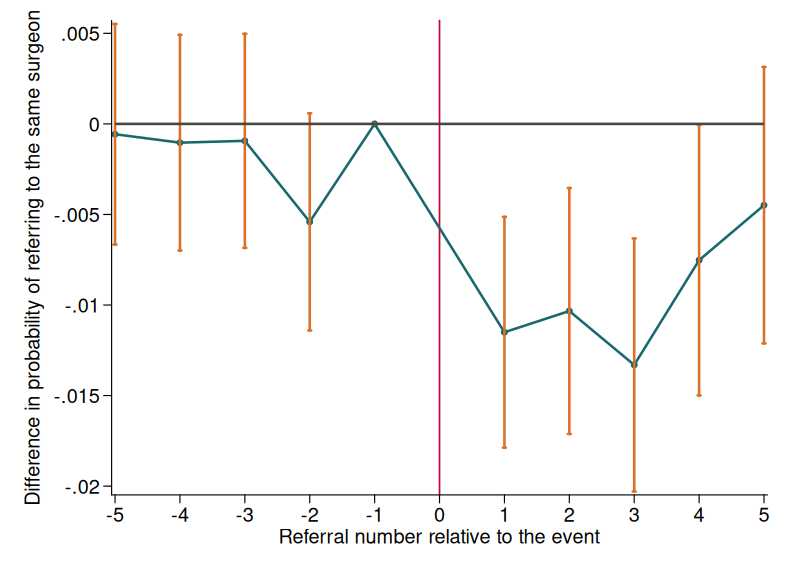
\includegraphics[scale=0.5]{results/figures/rf/Rereferral_EventStudy_1_1_0.png}
}
\label{fig:event}
\end{minipage}
\end{figure}

\clearpage
\section*{Change to Introduction}

To match the changes in our design-based evidence, we'd also need a change to the intro. This is what I have in mind. It would replace the event-study sentences in the introduction paragraph that begins ``Beyond this descriptive evidence.''

\medskip
\noindent We provide direct evidence of this behavior by comparing what a PCP does after referring a patient whose surgery ends in a failure with what the same PCP does after a referral that ends in a success. Relative to a success, a failure changes the probability that the PCP's next referral goes to the same specialist by $\rereferPct{}$ percent, and the relative response is largest for PCPs with little prior experience with that specialist, as Bayesian updating implies. This response is evidence of learning from the outcomes of a PCP's own patients, and it is precisely the variation that identifies the learning process in our structural model.

\clearpage
\section*{Change to Appendix}

I would also add a short section to the supplemental appendix that walks through the construction of the event study with an example. The proposed text follows.

\medskip
\section*{Construction of the Referral-Order Event Study}
\label{sec:app_es}

Every referral in our sample defines a window. The window consists of the referral itself, the PCP's five referrals before it, and the PCP's five referrals after it, indexed by $t=-5,\ldots,5$ with the defining referral at $t=0$. The specialist of the window is the one who received the referral at $t=0$, and the outcome at each other position is whether that referral went to the same specialist. A window is a failure window if the surgery at $t=0$ was a failure and a success window otherwise. Equation~\eqref{eqn:rereferral_es} compares the change in the outcome from the pre-period to the post-period between failure windows and success windows of the same PCP and of the same specialist and year.

Table~\ref{tab:app_es} illustrates with a PCP whose 22 referrals rotate among three specialists. The 22 referrals define 22 windows, seven for specialist 1 (centered on referrals 1, 4, 9, 11, 14, 17, and 20), seven for specialist 2, and eight for specialist 3, and the table shows three of them. Referral 6 goes to specialist 2 and fails. Every other referral succeeds. After the failure the PCP avoids specialist 2 for several referrals, so referrals 7 through 11 go to specialists 1 and 3, including referral 8, which would otherwise have gone to specialist 2, and the PCP first returns to specialist 2 at referral 13. The window centered on referral 6 is a failure window for specialist 2. Two of the five referrals in its pre-period went to specialist 2 and none of the five in its post-period did, and this change is the response that the event study measures.

Because every referral defines a window, each referral also lies in the windows of its neighbors, at a different position in each and compared with that window's specialist. Referral 8 is at position $+2$ in the window centered on referral 6, where the question is whether it went to specialist 2, and at position $-4$ in the window centered on referral 12, where the question is whether it went to specialist 3. The rows for one referral are therefore one choice recorded several times, and a referral that a failure diverted is a zero in the failure window and a one in a window for the specialist who received it instead.

We keep a window only if it contains no other failure. In the example, referral 6 lies in the windows centered on referrals 1 through 5 and 7 through 11, so all ten are dropped. These include the specialist 1 windows centered on referrals 1, 4, 9, and 11. The windows kept are the failure window and the success windows centered on referrals 12 through 22. The first success window kept after the failure is the one centered on referral 12, for specialist 3. This rule is blunt. It drops windows in which the failure sits at the edge and nothing in the window could have been affected, and in our data it keeps \rereferESEvents{} of \rereferEvents{} referrals as windows. Because the PCP fixed effects are interacted with position, a PCP contributes to the estimates only with at least one failure window and at least one success window.

The rule does not remove every window whose outcomes reflect the response. The pre-period of the window centered on referral 12 is referrals 7 through 11, the post-period of the failure window. Referral 8 is a zero in the failure window, because it did not go to specialist 2, and a one in the success window, because it went to specialist 3 instead, and both entries record the same response. The pre-period of the success window is elevated, three of five against one of five in its post-period, so its change of $-2/5$ matches the change in the failure window and the comparison between the two is zero. The success windows centered on referrals 13 through 16 have the same problem.

We therefore also estimate the event study after dropping any window that overlaps the post-period of another failure's window. In the example, the post-period of the failure window is referrals 7 through 11, and the windows centered on referrals 12 through 16 each contain some of them, so this drops those five windows, leaving the failure window and the success windows centered on referrals 17 through 22. The first of these windows is centered on referral 17, for specialist 1. Its pre-period and post-period each contain one referral to specialist 1, so its change is zero and the comparison recovers the $-2/5$ response. After this restriction no referral made while the PCP was responding to a failure appears in any success window. The dependence that remains across a PCP's windows involves referrals that no failure moved, and we account for it by clustering standard errors by PCP. In the data the overlap offsets only part of the response, and the restriction moves the estimate at the first referral after a failure from $\rereferESFirst{}$ to $\rereferESFirstSutva{}$.

\begin{table}[!ht]
\centering
\caption{Example of Overlapping Windows}
\label{tab:app_es}
\small
\begin{tabular}{ccccccccc}
\hline\hline
 & & & \multicolumn{2}{c}{Window 6} & \multicolumn{2}{c}{Window 12} & \multicolumn{2}{c}{Window 17} \\
 & & & \multicolumn{2}{c}{(specialist 2)} & \multicolumn{2}{c}{(specialist 3)} & \multicolumn{2}{c}{(specialist 1)} \\
Referral & Specialist & Outcome & Position & Same & Position & Same & Position & Same \\
\hline\hline
1 & 1 & S & $-5$ & 0 & & & & \\
2 & 2 & S & $-4$ & 1 & & & & \\
3 & 3 & S & $-3$ & 0 & & & & \\
4 & 1 & S & $-2$ & 0 & & & & \\
5 & 2 & S & $-1$ & 1 & & & & \\
6 & 2 & F & 0 & & & & & \\
7 & 3 & S & 1 & 0 & $-5$ & 1 & & \\
8 & 3 & S & 2 & 0 & $-4$ & 1 & & \\
9 & 1 & S & 3 & 0 & $-3$ & 0 & & \\
10 & 3 & S & 4 & 0 & $-2$ & 1 & & \\
11 & 1 & S & 5 & 0 & $-1$ & 0 & & \\
12 & 3 & S & & & 0 & & $-5$ & 0 \\
13 & 2 & S & & & 1 & 0 & $-4$ & 0 \\
14 & 1 & S & & & 2 & 0 & $-3$ & 1 \\
15 & 3 & S & & & 3 & 1 & $-2$ & 0 \\
16 & 2 & S & & & 4 & 0 & $-1$ & 0 \\
17 & 1 & S & & & 5 & 0 & 0 & \\
18 & 3 & S & & & & & 1 & 0 \\
19 & 2 & S & & & & & 2 & 0 \\
20 & 1 & S & & & & & 3 & 1 \\
21 & 3 & S & & & & & 4 & 0 \\
22 & 2 & S & & & & & 5 & 0 \\
\hline\hline
\end{tabular}
\begin{minipage}{6in}
\vspace{1ex}
\footnotesize One PCP's 22 referrals in order, with the specialist who received each and its surgical outcome (S for success, F for failure). Every referral defines a window, so these referrals define 22 windows; the table shows three of them. Each window is named for the referral at its position 0, and its specialist is the one who received that referral. Position is the referral's position in the window, and Same is one if the referral went to the window's specialist. Window 6 is a failure window; windows 12 and 17 are success windows. Referrals 7 through 11 are the post-period of window 6 and the pre-period of window 12.
\end{minipage}
\end{table}

\end{document}
